% !TeX spellcheck = fr
% !TeX encoding = UTF-8
\documentclass{beamer}

\usepackage{fontspec}
\usepackage{xltxtra}

%\usetheme{Boadilla}
\usetheme{PaloAlto}
%\usetheme{Berlin}
%\usecolor{}

\usepackage{minted}

%\setmainfont{Linux Libertine O}
\usepackage[english,french]{babel}

%Un peu de config de Beamer
\setbeamersize{description width=0.47cm}


\usepackage{hyperref}

\usepackage{graphicx}

\institute{Univ. de Neuchâtel}

\title{Exploiter les données}
\subtitle{Introduction à la textométrie avec \textsc{txm}}
\author{Jean-Baptiste Camps \& Simon Gabay}
\date[FoPhil -- 14 févr. 2018]{Formation en philologie numérique:\\ encoder, exploiter, diffuser\\
12-16 février 2018}

\makeatletter 
         
        \AtBeginSection[]{% 
        \begin{frame}{Plan}%
        \small
        \tableofcontents[currentsection]%
        \end{frame} }

        %\AtBeginSubsection[]{% 
	%\begin{frame}{Plan}%
	%\small
	%\tableofcontents[currentsection,currentsubsection]%
%\end{frame} }


\makeatother 
    
    
\begin{document}

\maketitle
%\frontmatter 
  

\begin{frame}{De la production des données à l'exploitation}
	
	\begin{columns}[T]
		
		\begin{column}{0.62\textwidth}
			
			\textsc{Ceux-ci collectent les données}
			
			\centering
			
			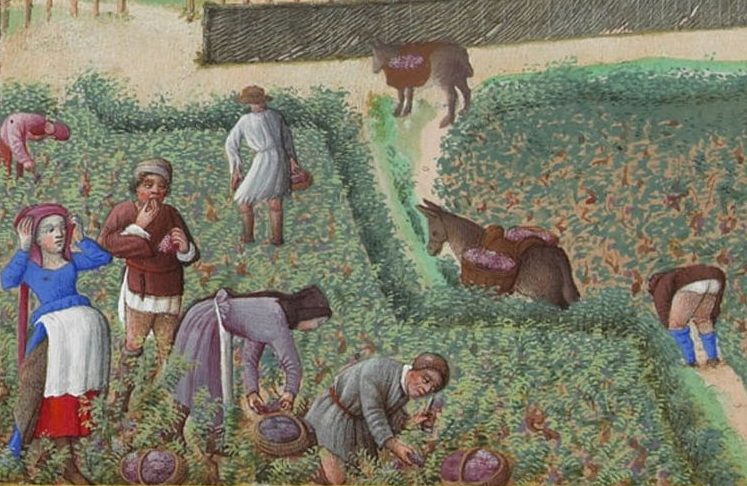
\includegraphics[width=\textwidth]{img/vendange.jpg}
			
		\end{column}
			\begin{column}{0.38\textwidth}
		
		\textsc{Ceux-là les exploitent}
		
		\centering
		
		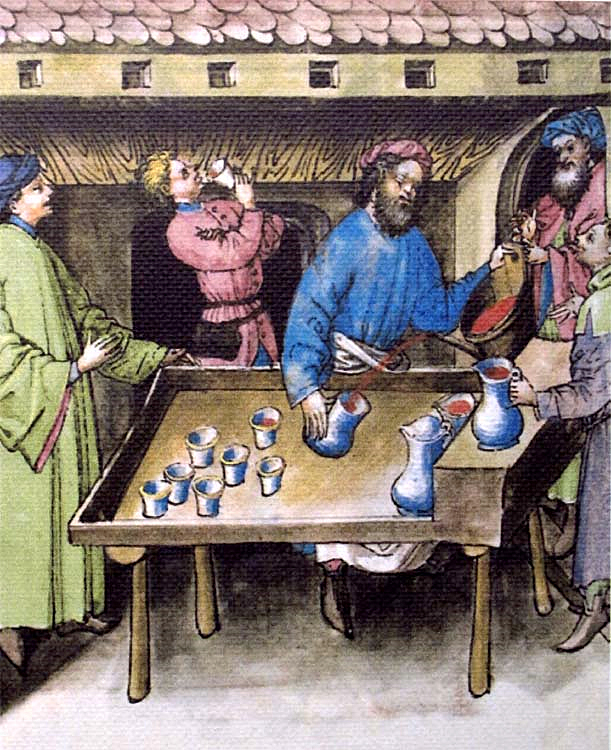
\includegraphics[width=\textwidth]{img/vin2.jpg}
		
	\end{column}
		
	\end{columns}
	
\end{frame}

%\mainmatter 

\begin{frame}{Objectifs}
	
	\begin{itemize}
		\item S'initier à la \alert{textométrie},
		\begin{itemize}
			\item créer des corpus;
			\item les interroger;
			\item faire (un peu) d'analyse quantitative.
		\end{itemize}
		\item dans le cadre d'un logiciel ``tout en un'' et convivial, 
	\alert{\textsc{txm}} \cite{Heiden2010},
		\item sur des cas tirés de la littérature du XVII\ieme{} siècle.
	\end{itemize}


\begin{block}{La textométrie selon \cite{Pincemin2008}}
	\begin{quote}
		La   textométrie développe  les  possibilités  de  consultation  et  d'analyse  de
		corpus  textuels  en  faisant  appel  à  des  décomptes  et des
		modélisations  statistiques  et  en  combinant  aux  possibilités
		de repérage d'occurrences des calculs de tri, de sélection et
		de réorganisation statistique.
	\end{quote}
\end{block}
	
\end{frame}


\begin{frame}[fragile]
\frametitle{\textsc{txm}: un logiciel de textométrie}


\begin{columns}
	\begin{column}{0.30\textwidth}
	\begin{center}
	
\includegraphics[width= 0.8\textwidth]{img/txm.png}
	\end{center}

\url{http://textometrie.ens-lyon.fr/}

\textit{Base de français médiéval:} \url{http://txm.bfm-corpus.org/}.
	\end{column}
	\begin{column}{0.66\textwidth}
		\begin{itemize}
			\item Logiciel libre et multiplateforme;
			\item développé à l'ÉNS-LSH de Lyon;
			\item dévoué à la textométrie;
			\item repose sur des technologies de référence:
				\begin{itemize}
					\item \textsc{xml/tei} pour les données;
					\item \textsc{r} pour l'analyse statistique;
					\item \textsc{cqp} pour l'interrogation de corpus;
					\item \texttt{TreeTagger} pour l'annotation.
				\end{itemize}
		\end{itemize}
	\end{column}
\end{columns}
\end{frame}


\begin{frame} 
  \frametitle{Plan} 
  \tableofcontents
\end{frame}

\section{Mise en jambe: \textit{Andromaque}}

\begin{frame}{Création d'un corpus à partir de notre édition d'\textit{Andromaque}}

\begin{enumerate}
	\item Fichier, importer, import XML/W + CSV;
	\item sélectionner le dossier avec les sources et remplir les paramètres du corpus;
	\item lancer la création du corpus.
\end{enumerate}

\end{frame}

\begin{frame}{Premières fonctionnalités}
\begin{enumerate}
\item Consulter la description du corpus;
\item parcourir l'édition;
\item regarder le lexique;
\item ouvrir l'index, y chercher les occurrences de 'Seigneur';
	\begin{enumerate}
		\item clic-droit, envoyer vers les concordances;
			\begin{enumerate}
				\item double-clic sur une occurrence pour aller au texte;
			\end{enumerate}
		\item clic-droit, envoyer vers les cooccurrents;
			\begin{enumerate}
				\item aller d'un cooccurrent aux concordances, puis au texte
			\end{enumerate}
		\item clic-droit, envoyer vers la progression;
	\end{enumerate}
\end{enumerate}

\end{frame}

\begin{frame}{Partitions et quelques éléments descriptifs}
\begin{enumerate}
\item créer une partition, en sélectionnant la structure \texttt{sp} et l'attribut \texttt{\@who};
\item consulter les dimensions;
\item créer une table lexicale, expérimenter avec les tris, la fusion ou suppression des colonnes, etc.
\end{enumerate}
\end{frame}

\begin{frame}{Statistiques de base}
À partir de la table lexicale créée,
\begin{enumerate}
\item calculer les spécificités;
\item quels sont les mots les plus spécifiques d'Oreste? de Pylade?
\item en sélectionner quelques uns qui sont pertinents;
\item calculer le diagramme en bâton des lignes sélectionnées.
\end{enumerate}
\end{frame}

\begin{frame}{Qu'en déduire?}
	
	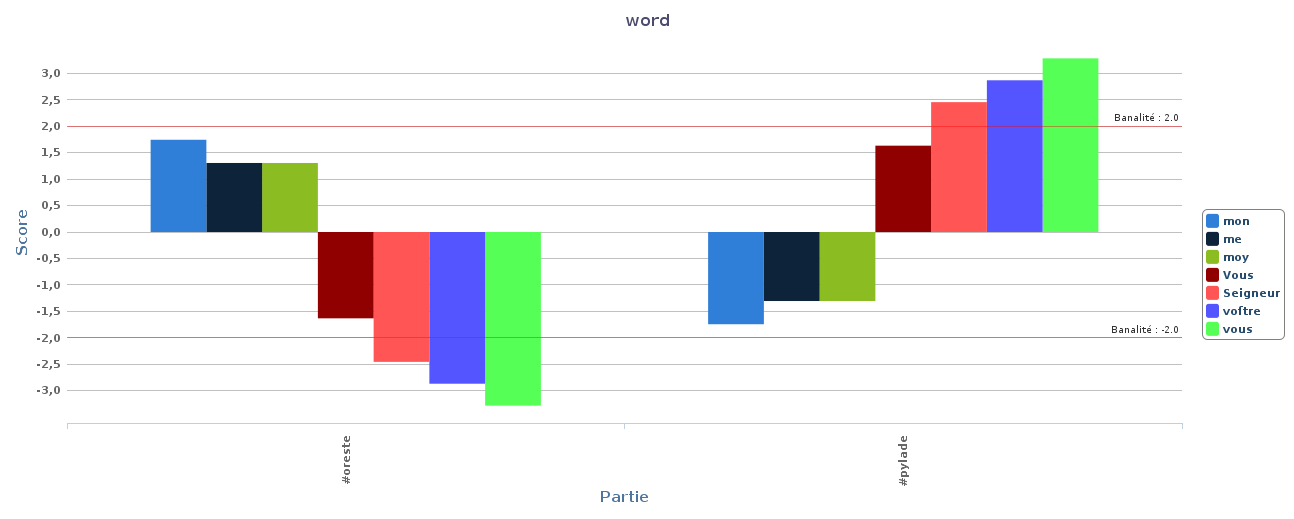
\includegraphics[width=\textwidth]{img/graphique_word_Oreste.png}
	
\end{frame}

%TODO: ajouter formule et expliquer maths des spécificités, si temps.


\frame{Prêts à passer aux choses sérieuses?}

\section{Importer des données et créer un corpus}

\begin{frame}{Différents modes d'import}
	
	\begin{description}
		\item[flemmards] import (avec ou sans métadonnées complémentaires)
		depuis 
		\begin{itemize}
			\item presse-papier;
			\item des fichiers \texttt{txt} ;
			\item traitement de texte.
		\end{itemize}
		\item[XML] XML/ TEI ou autre;
		\item[spécifiques] formats de logiciels de textométrie.
	\end{description}
	
\end{frame}

% Le corpus

\begin{frame}[fragile]
\frametitle{Corpus du jour: un peu de théâtre du XVII\ieme{} siècle}

Corpus constitué pour le cours d'aujourd'hui:

\begin{itemize}
	\item source: Paul Fièvre,  \url{http://www.theatre-classique.fr/};
	\item documents encodés en \textsc{xml}/\textsc{tei} (ou dans plusieurs \textsc{xml/tei});
	\item corpus de \alert{36} pièces de théâtre en vers du XVII\ieme{} siècle,
	\item appartenant à trois genres principaux:
		\begin{itemize}
			\item comédie,
			\item tragédie,
			\item tragi-comédie.
		\end{itemize}
	\item sélectionnées un peu au hasard,
	\begin{itemize}
		\item mais en essayant de conserver un équilibre entre les genres principaux (comédie, tragédie, tragi-comédie),
		\item d'avoir des pièces de longueur similaire (entre 1250 et 2000 vers),
		\item un équilibre entre les auteurs (4 pièces par auteur),
		\item et entre les générations (4 auteurs par génération).
	\end{itemize}
\end{itemize}

\end{frame}

\begin{frame}{9 auteurs, 2 générations}
	%	Auteurs, approximativement de deux générations un peu différentes du XVII\ieme{} siècle,
	\begin{columns}[T]
		\begin{column}{0.45\textwidth}
			G1, c.~1630-1650
			\begin{itemize}
			    \item Pierre Du Ryer \\(fl. 1628-1655);
			    \item Georges de Scudéry\\ (fl. 1631-1643).
				\item Jean de Rotrou\\ (fl. 1635-1649);
				\item Paul Scarron\\ (fl. 1648-1660);
			\end{itemize}
		\end{column}
		\begin{column}{0.45\textwidth}
			G2, c.~1650-1690
			\begin{itemize}
				\item Claude Boyer\\ (fl. 1646-1697);
				\item Thomas Corneille\\ (fl. 1651-1696)
				\item Molière\\ (fl. 1655-1673)
				\item Jean Racine\\ (fl. 1664-1691);
			\end{itemize}
		
		\end{column}
	\end{columns}
	
			Et un monstre sacré, \textbf{Pierre Corneille} (fl. 1629-1675).
	
\end{frame}

\begin{frame}{Sources et pré-traitements}
	
	
	 \begin{itemize}
	 	\item Graphies modernisées (dommage… mais va faire notre affaire dans ce cas précis);
	 	\item Faut-il supprimer la distinction majuscule/minuscule?
	 		\begin{itemize}
	 			\item Pour: suppression de biais éditoriaux.
	 			\item Contre: les majuscules peuvent conserver de l'information syntaxique.
	 		\end{itemize}
 		\item Veut-on garder tout ce qui est extérieur aux répliques (liste des personnages, page de titre, etc.)?
 			\begin{itemize}
 				\item Peut être retiré grâce à la structuration \textsc{xml/tei}.
 			\end{itemize}
	 	\item pas de lemmatisation: possibilité de lemmatiser et annoter automatiquement.
	 \end{itemize}
	
\end{frame}

\begin{frame}[fragile]
\frametitle{Transformations avant l'import}
	
	Dossier \texttt{xsl}, feuille \texttt{source\_to\_txt.xsl} (2.0), deux sorties:
	
	\begin{enumerate}
		\item fichier \texttt{metadata.csv}: métadonnées des documents extraites automatiquement des fichiers \textsc{tei} (\texttt{teiHeader} et page de titre, \texttt{docDate});
		\item dossier \texttt{txt}: transformation en \texttt{txt} des pièces:
			\begin{itemize}
				\item passage en bas de casse;
				\item suppression du \texttt{teiHeader};
				\item suppression du \texttt{castList} et des mentions de personnage, \texttt{speaker};
				\item suppression du \texttt{front}, des \texttt{docTitle}, \texttt{docDate}, \texttt{docAuthor}, \texttt{docImprint}, \texttt{printer}, \texttt{performance}, \verb|div[\@type='dedicace']|;
				\item suppression des titres, notes.
			\end{itemize}
	\end{enumerate}
	
\end{frame}

\begin{frame}{Import \texttt{txt} + \texttt{csv}}
	
	\begin{enumerate}
		\item sélectionner le répertoire de sources \texttt{txm\_import1\_txt} (contenant fichiers \texttt{txt} et métadonnées \texttt{csv},
		corpus tronqué pour gagner un peu de temps);
		\item paramétrer l'import (nommer le corpus THEATRENEUCHTXT);
		\item demander la lemmatisation;
		\item vérifier que les métadonnées sont bien comprises;
		\item lancer l'import;
		\item (regarder le log de l'import);
		\item une fois l'import réussi, jeter un œil à la description, à l'édition, etc.
	\end{enumerate}
	
\end{frame}

% Import XML amélioré, avec XSLT intermédiaire, lemmatisation, etc. etc.

\begin{frame}{Import \texttt{xml/w} + \texttt{csv} amélioré}

\begin{enumerate}
	\item sélectionner le répertoire de sources \texttt{txm\_import2\_xml} (contenant fichiers \texttt{xml} et métadonnées \texttt{csv},
complet);
	\item paramétrer l'import (nommer le corpus THEATRENEUCHXML);
	\item demander la lemmatisation;
	\item vérifier que les métadonnées sont bien comprises;
	\item \alert{associer l'\texttt{xsl} 2.0 de pré-traitement, \texttt{import\_xml\_filtre.xsl}};
	\item lancer l'import;
	\item (regarder le log de l'import);
	\item une fois l'import réussi, jeter un œil à la description, à l'édition, etc.
\end{enumerate}

\end{frame}


\section{Interroger les données}

\begin{frame}{\textsc{cqp} et \textsc{cql}}
	
	\begin{block}{Corpus Query Processor}
		Composant logiciel qui traite des requêtes:\\
		moteur de recherche qui permet de trouver toutes les occurrences
		correspondant à une requête.
		
		\begin{itemize}
			\item logiciel libre;
			\item développé initialement à l'Univ. de Stuttgart;
			\item \url{http://cwb.sourceforge.net/}.
		\end{itemize}
		
	\end{block}

	\begin{block}{Corpus Query Language}
		Langage d'expression de requêtes (cf. SQL, XQuery…).\\
		Une expression CQL est une chaîne de caractères exprimant un motif
		linguistique (un mot, ou une suite de mots) à partir des valeurs de leurs propriétés (comme la
		catégorie grammaticale, le lemme, la forme graphique). (voir Manuel de TXM).
	\end{block}
	
\end{frame}

\begin{frame}{Interroger avec \textsc{txm}: niveau 0}
	
	Entrer un mot dans le champ de l'interface \texttt{Index}.
	
	Ex. 'seigneur'.
	
\end{frame}

\begin{frame}{Interroger avec \textsc{txm}: niveau 1, assistant}

Cliquer sur la baguette magique, pour accéder à l'assistant de création de requêtes

Chercher:
\begin{itemize}
	\item la forme 'seigneur',
	\item suivie d'un pronom (cf. la doc, \\ \texttt{JeuEtiquettesModeleFrancaisTreeTagger.pdf}),
		\begin{itemize}
			\item astuce: commence par 'PRO'
		\end{itemize}
	\item suivi de n'importe quelle forme du lemme 'être'.
\end{itemize}

%TODO: screenshot (déjà enregistré)

\end{frame}

\begin{frame}{Interroger avec \textsc{txm}: niveau 2, un peu de \textsc{cql}}
	
	En \textsc{cql}, la requête précédente correspond à:\\
	\texttt{[word="seigneur"][frpos="PRO.*"] [frlemma="être"] }
	
	On se lance:
	\begin{enumerate}
		\item Modifier la requête pour permettre un mot, quel qu'il soit, entre seigneur et le pronom;
		\item la modifier, pour limiter aux cas où ce mot est une virgule;
		\item l'éditer pour étendre aux cas où ce mot est une virgule OU un point d'interrogation.
	\end{enumerate}
	
\end{frame}


\begin{frame}{Interroger avec \textsc{txm}: niveau 3, \textsc{cql} (plus) avancé}

\begin{columns}
	\begin{column}{0.48\textwidth}
		
		\begin{block}{Ignorer:}
			\begin{description}
				\item[\texttt{\%c}] casse, ex. \texttt{[word="état"\%c]}
				\item[\texttt{\%d}] diacritiques, ex. \texttt{[word="état"\%d]}
				\item[\texttt{\%d}] les deux, ex., \texttt{[word="état"\%cd]}
			\end{description}
		\end{block}

		\begin{block}{Opérateurs:}
			\begin{description}
				\item[=] égal
				\item[!=] différent
				\item[|] ou
				\item[\&] et
				\item[()] priorité des opérations
			\end{description}
		\end{block}		
		
	\end{column}
	\begin{column}{0.48\textwidth}
	
	\begin{block}{Quantificateurs}
		\begin{description}
			\item[mot] mot une seule fois (1);
			\item[mot+] mot une seule fois ou plus (1…n);
			\item[mot?] mot 0 ou une fois (0…1);
			\item[mot*] mot 0 fois ou plus (0…n);
			\item[mot\{2,4\}] mot entre 2 et 4 fois (2…4);
		\end{description}
	\end{block}
		
	\end{column}
\end{columns}


\end{frame}


\begin{frame}{Interroger avec \textsc{txm}: niveau 3, (suite)}

\begin{columns}
	\begin{column}{0.48\textwidth}
		
		\begin{block}{Échapper des caractères spéciaux}
			
			Pour entrer '?', '*', '.', '+', '|', '\&', …, qui sont des caractères spéciaux,\\
			les \textbf{faire précéder d'une barre oblique inverse}. Ex.,\\
			\texttt{\textbackslash?}
			
		\end{block}
		
	\end{column}
	\begin{column}{0.48\textwidth}
		
		
		\begin{block}{Classes de caractères}
		
		\begin{description}
			\item[.] n'importe quel caractère;
			\item[{[mn]}] un m ou un n;
			\item[{[a-z]}] une minuscule non accentuée;
			\item[{[\^~a-z]}] tout sauf … ;
			\item[\textbackslash{}d] un chiffre;
			\item[\textbackslash{}s] un caractère d'espacement;
			\item[\textbackslash{}w] un caractère de mot;
			\item[\textbackslash{}D] tout sauf un chiffre;
			\item[\textbackslash{}S] tout sauf un car. d'espacement;
			\item[\textbackslash{}W] tout sauf un car. de mot;
		\end{description}
		\end{block}
		
		
	\end{column}
\end{columns}


\end{frame}


\begin{frame}{Interroger avec \textsc{txm}: niveau 3, exercices}

\begin{enumerate}
	\item un mot contenant un chiffre.
	\item une forme commençant par 'a' et finissant par 'er';
	\item une forme de deux lettres: une voyelle et 'h';
	\item 'seigneur' ou 'dame', suivi ou non d'un mot et suivi d'un pronom (n'importe quel type de pronom).
	\item la forme 'je', suivie d'entre 2 et 4 mots, et d'une virgule.
\end{enumerate}

\end{frame}


\begin{frame}[fragile]
\frametitle{Interroger avec \textsc{txm}: niveau 4, \textsc{cql} \emph{hardcore}}
		
		\begin{block}{Expressions régulières plus avancées}
			\textbf{Classes de caractères Unicode}
			\begin{description}
				\item[\textbackslash{}p\{Lu\}] une majuscule (au sens de la propriété Unicode);
				\item[\textbackslash{}p\{P\}] une majuscule (au sens de la propriété Unicode);
				\item[\textit{etc.}]
			\end{description}
		\end{block}
		
		N.B.: \alert{Toutes les PCRE (Perl-Compatible Regular Expressions) sont disponibles dans \textsc{cql}}. 
		Voir  \href{http://regexkit.sourceforge.net/Documentation/pcre/pcrepattern.html}{\textcolor{blue}{la doc}}.
		
		%within, expand to, …
		
		\begin{block}{Instructions de \textsc{cql}}
			
			On peut limiter la zone de recherche en utilisant \texttt{within}.
			Ex. \\
			\verb|[word="et"][]*[word="je"] within 10|\\
			'et … je', dans une limite de 10 mots\\
			\verb|[word="et"][]*[word="je"] within l|\\
			'et … je', dans un vers.
		\end{block}

\end{frame}

\begin{frame}[fragile]
\frametitle{Interroger avec \textsc{txm}: niveau 4, suite}

\begin{block}{Utiliser les propriétés de structure}
	Possible d'utiliser les propriétés de structure et \textsc{xml} pour préciser les requêtes.
	
	\verb|<l> [frpos="VER.*"] [] * </l>|\\
	Vers commençant par un verbe.
	
	\verb|<l>  [] * [word=".*uite"] </l>|\\
	Vers ayant 'uite' à la rime.
	
\end{block}

\textit{Want more?} La \href{http://cwb.sourceforge.net/documentation.php}{\textcolor{blue}{doc de CQL}} est pour vous, ainsi que le 
\href{http://txm.sourceforge.net/doc/manual/manual1.xhtml}{\textcolor{blue}{manuel de TXM}}.

\end{frame}

\begin{frame}{Interroger avec \textsc{txm}: niveau 4, exercices}

\begin{enumerate}
	\item une forme contenant de la ponctuation;
	\item un vers d'entre 4 et 5 mots;
	\item un vers débutant par un pronom personnel (\texttt{PRO:PER}) débutant par 't';
	\item un vers se terminant par '-ron' (suivi ou non d'une consonne).
\end{enumerate}

\end{frame}

\section{Quelques notions d'analyse quantitative}

\begin{frame}[fragile]
\frametitle{Deux approches: la forme (style) ou le fond (sémantique)?}

\begin{description}
	\item[stylométrie] attribution, datation, localisation des textes. 
		\begin{itemize}
			\item information graphique, flexionnelle, etc. 
			\item \alert{mots les plus fréquents} (mots-outils, mots-vides), moins sensibles aux variations intentionnelles de leurs auteurs (genre, sujet, etc.).
		\end{itemize}
	\item[approche sémantique] (lexicométrie, lecture distante,…), à peu près l'inverse de la précédente: 
		\begin{itemize}
			\item lemmes;
			\item cooccurrents;
			\item mots plus rares.
		\end{itemize}
\end{description}

\end{frame}

\begin{frame}{Un peu d'exploration du corpus}
	
	Vérifions tout d'abord si le corpus est bien équilibré, et étudions les distributions par:
	\begin{itemize}
		\item genre;
		\item auteur;
		\item période
		\item taille des textes.
	\end{itemize}

Pour ce faire:
\begin{enumerate}
	\item créer une partition pour chacune de ces questions, grâce aux métadonnées de \texttt{text};
	\item observer les \texttt{dimensions}.
\end{enumerate}
	
\end{frame}


%Partitions par genre, auteur, texte. Table-lexicale, lemmes ou formes

\begin{frame}{Un peu d'exploration des genres}
	
	\begin{block}{Thématique}
		
		\begin{enumerate}
			\item créer une table lexicale (idéalement, des lemmes) de la partition genre, des 500 formes les plus fréquents;
			\item la traiter pour retirer les mots vides;
			\item calculer les spécificités, sélectionner pour mettre en valeur les particularités de la tragédie, créer le graphique;
			\item calculer la classification;
			\item calculer l'AFC.
		\end{enumerate}
	\end{block}

\begin{block}{Stylistique}
	
	\begin{enumerate}
		\item créer une table lexicale des formes de la partition genre, des 200 formes les plus fréquentes;
		\item la traiter pour retirer les mots porteurs de sens;
		\item calculer la classification;
		\item calculer l'AFC.
	\end{enumerate}
\end{block}
	
\end{frame}


\begin{frame}{(Quelques) lemmes spécifiques de la tragédie}
	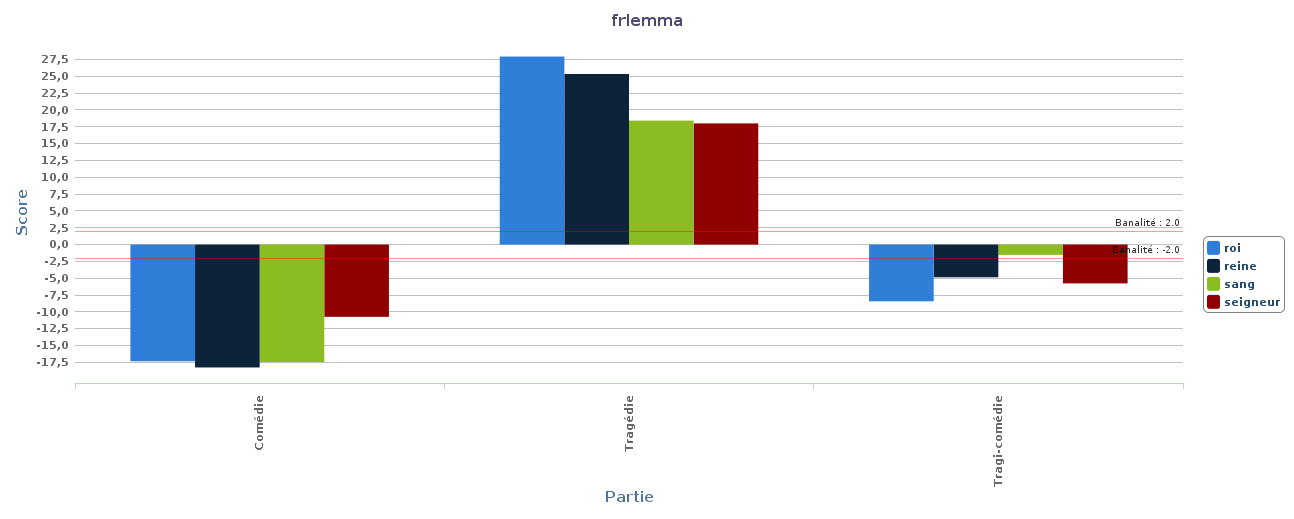
\includegraphics[width=\textwidth]{img/Graphique_genre_frlemma_specif.png}
\end{frame}


\begin{frame}{Problématiques autoriales}
	Passons maintenant aux choses sérieuses et aux questions d'attribution.
	
	\textbf{Étape 1: observer la répartition des auteurs}
	
	Sur la partition par auteurs,
	\begin{enumerate}
		\item Créer une table lexicale des 200 formes les plus fréquentes, retirer les mots porteurs de sens;
		\item calculer les spécificités, et les étudier pour voir quels auteurs ont des tics très marqués;
		\item calculer la classification;
		\item calculer l'AFC.
	\end{enumerate}
	
\end{frame}

\begin{frame}{(Quelques) tics de langage de Claude Boyer}
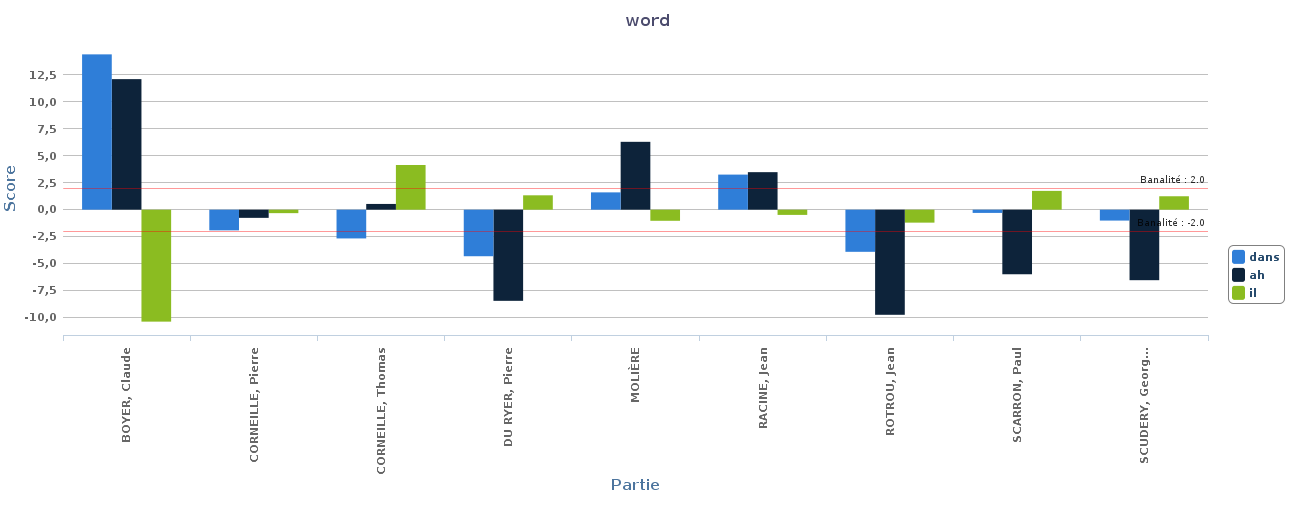
\includegraphics[width=\textwidth]{img/Graphique_word_parAuteurs_specif.png}
\end{frame}

\begin{frame}{L'Analyse factorielle des correspondances}
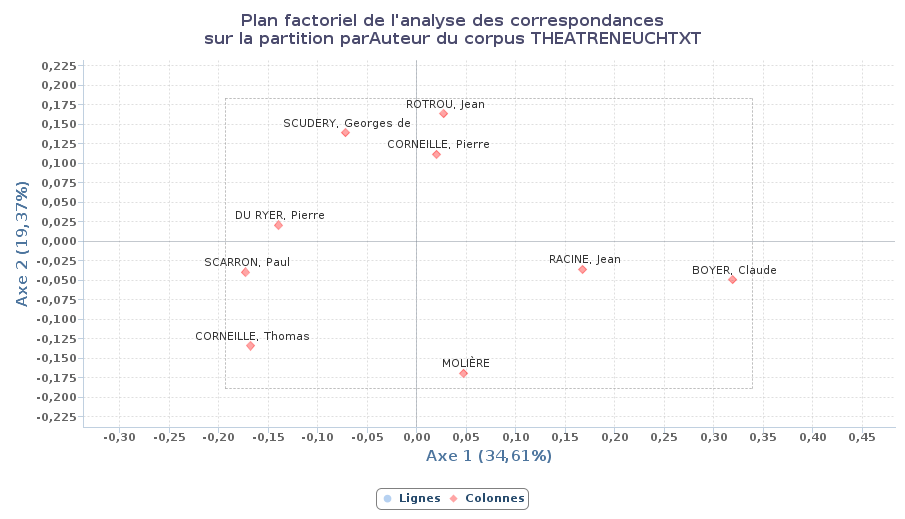
\includegraphics[width=\textwidth]{img/parAuteur_word_AFC_1-2.png}
\end{frame}

\begin{frame}{Une répartition surtout chronologique}
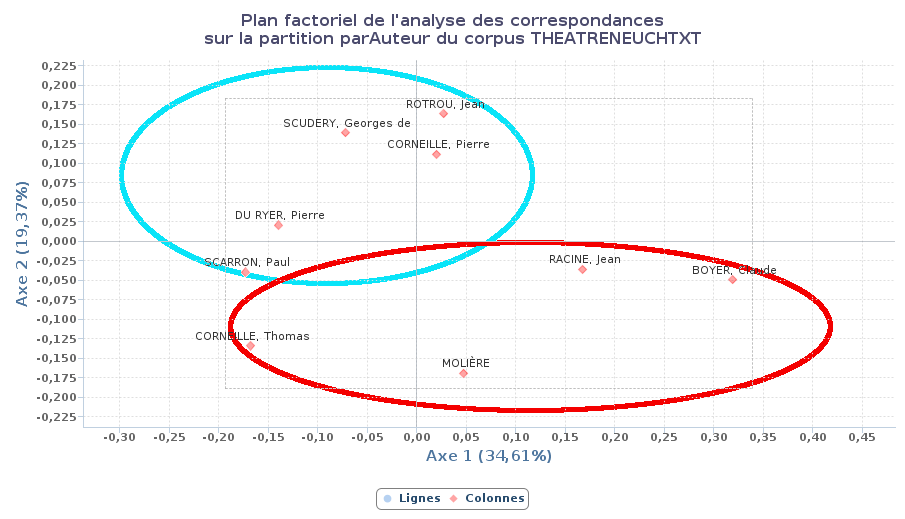
\includegraphics[width=\textwidth]{img/parAuteur_word_AFC_1-2_edit.png}
\end{frame}

% Problématique: les auteurs (stylométrie)

\begin{frame}{Et maintenant: les textes eux-mêmes…}

	Sur la partition par textes,
\begin{enumerate}
	\item Créer une table lexicale des 200 formes les plus fréquentes, retirer les mots porteurs de sens;
	\item calculer la classification;
	\item calculer l'AFC.
\end{enumerate}

\end{frame}


\frame{
	\vspace{0.3\textheight}
\begin{center} 
	\Large \textsc{to be continued}…\\
	Avec R.
	
\end{center}

}


\appendix

\section{Solutions des exercices}

\begin{frame}{Solutions}{Interroger avec \textsc{txm}: niveau 2, un peu de \textsc{cql}}

\begin{enumerate}
	\item Modifier la requête pour permettre un mot, quel qu'il soit, entre seigneur et le pronom;\\
	\texttt{[word="seigneur"][][frpos="PRO.*"] [frlemma="être"]}
	\item la modifier, pour limiter aux cas où ce mot est une virgule;\\
	\texttt{[word="seigneur"][word=','][frpos="PRO.*"] [frlemma="être"] }
	\item l'éditer pour étendre aux cas où ce mot est une virgule OU un point d'interrogation.\\
	\texttt{[word="seigneur"][word=',' | word='\textbackslash?'][frpos="PRO.*"] [frlemma="être"] }
\end{enumerate}

\end{frame}

\begin{frame}[fragile]
\frametitle{Solutions}
\framesubtitle{Interroger avec \textsc{txm}: niveau 3, exercices}

\begin{enumerate}
	\item un mot contenant un chiffre.\\
	\texttt{[word=".*\textbackslash{}d.*"]}
	\item une forme commençant par 'a' et finissant par 'er';\\
	\texttt{[word="[a].*er"]}
	\item une forme de deux lettres: une voyelle et 'h';\\
	\texttt{[word="[aeiouy]h"]}
	\item 'seigneur' ou 'dame', suivi ou non d'un mot et suivi d'un pronom (n'importe quel type de pronom).\\
	\texttt{[word="seigneur" | word="dame"][]?[frpos="PRO.*"]}
	\item la forme 'je', suivie d'entre 2 et 4 mots, et d'une virgule.\\
	\texttt{[word="je"][]{2,4}[word=","]}
\end{enumerate}

\end{frame}

\begin{frame}[fragile]
\frametitle{Solutions}
\framesubtitle{Interroger avec \textsc{txm}: niveau 4, exercices}

\begin{enumerate}
	\item une forme contenant de la ponctuation;\\
	\verb|[word=".*\p{P}.*"]}|
	\item un vers d'entre 4 et 5 mots;\\
	\verb|<l>  []{4,5} </l>|
	\item un vers débutant par un pronom personnel (\texttt{PRO:PER}) débutant par 't';\\
	\verb|<l>  [word="t.*" & frpos="PRO:PER"] []* </l>|
	\item un vers se terminant par '-ron' (suivi ou non d'une consonne).\\
	\verb|<l>  [] * [word=".*ron[^aeiou]"] </l>|
\end{enumerate}

\end{frame}

%TODO: quelques explications stats AFC et CAH

\section{Explications mathématiques}
\subsection{AFC}



\begin{frame}[fragile]
\frametitle{Analyse par réduction des dimensions}

\begin{itemize}
	\item Nous avons vu lors du cours précédent comment des représentations graphiques simples permettaient de résumer une grande partie de la relation entre deux variables.
	\item L'objectif des méthodes d'analyse de données que nous allons présenter est de remplir les mêmes offices dans le domaine plus délicat des statistiques multivariées.
	\item Ces analyses de données, qui visent à simplifier l'information pour la rendre lisible, sont appelées \alert{analyse par réduction des dimensions}.
	\item Au-delà d'usages descriptifs que nous évoquerons ici, certaines de ces méthodes ont un usage prédictif. Elles feront l'objet de notre dernière séance.
\end{itemize}

\end{frame}

\begin{frame}[fragile]
\frametitle{Analyse par réduction des dimensions: objectifs}

La valeur de ces méthodes est pour nous triple:

\begin{itemize}
\item \textbf{Visualiser} des données complexes pour y discerner des regroupements, des régularités, des typologies
\item \textbf{Débruiter} les données, en supprimant de l'analyse les dimensions qui peuvent être considérées comme à négliger
\item \textbf{Décorréler}: les axes créés au cours de ces analyses ne sont pas nécessairement des variables de la base, mais des construits n'ayant aucune corrélation entre eux.
\end{itemize}

\end{frame}

\begin{frame}[fragile]
\frametitle{Analyse par réduction des dimensions: méthode}



\begin{itemize}
\item Dans une analyse factorielle, on cherche à déterminer les axes qui absorbent le plus d’inertie possible par rapport au centre de gravité du nuage de point.
\item Concrètement, on va passer d'un nuage de points de grande dimension à un sous-espace de plus petite dimension, sur lequel on pourra réunir la plus grande quantité d'information possible. 
\item On choisit de déterminer des axes, définissant un plan sur lequel les points du nuage seront projetés. 
\item Ces axes sont choisis pour que les points projetés soient les plus dispersés possibles.
\end{itemize}
\end{frame}


\begin{frame}[fragile]
\frametitle{Analyse par réduction des dimensions: typologie}

\begin{center}
%\vspace{-3em}
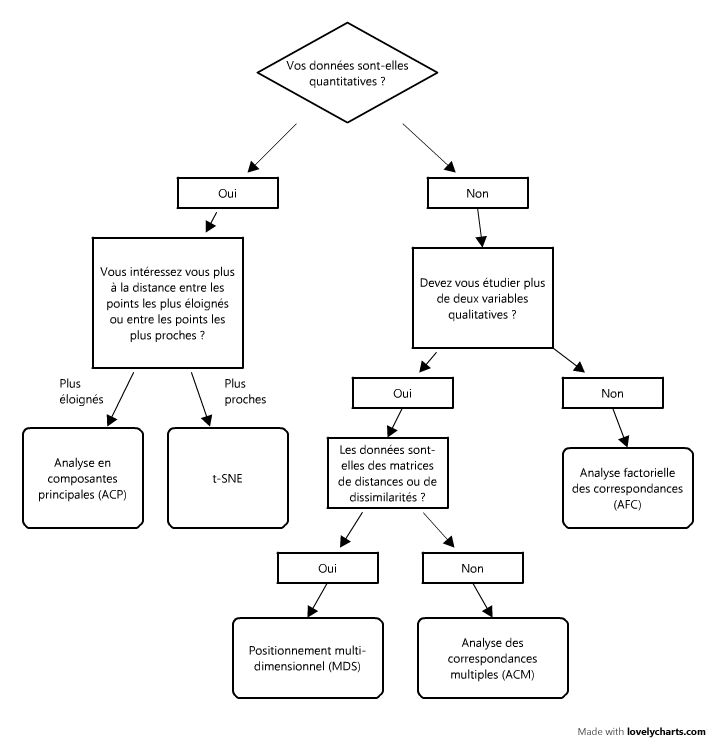
\includegraphics[height=8.6 cm]{img/af.png}
\end{center}

\end{frame}

\begin{frame}[fragile]
\frametitle{Analyse par réduction des dimensions: typologie}

Trois de ces méthodes sont particulièrement usitées. Elles sont utiles dans des circonstances différentes: 
\begin{enumerate}
\item Quand les variables sont quantitatives, on peut réaliser une \alert{Analyse en Composantes Principales (ACP)}.
\item Quand les variables sont qualitatives, on utilise des \alert{Analyses des Correspondances} - la correspondance étant "l'équivalent" de la corrélation pour des variables qualitatives:
\begin{itemize}
\item Quand les individus sont décrits par deux variables qualitatives, on peut construire un tableau de contingence et réaliser une \alert{Analyse Factorielle des Correspondances (AFC)}. 
\item Quand les individus sont décrits par un jeu plus de deux variables qualitatives, on peut réaliser une \alert{Analyse des Correspondances Multiples (ACM)}.
\end{itemize}

\end{enumerate}
\end{frame}

\begin{frame}[fragile]

\frametitle{Analyse par réduction des dimensions: ventilation}

\begin{itemize}
\item Nécessité parfois de se débarrasser de modalités peu pertinentes, car elles brouillent le calcul, ou la visualisation
\item Plutôt que la suppression, possibilité de ventiler: on remplace les modalités ne dépassant pas un effectif minimal par la valeur moyenne de l'échantillon sans ces modalités. On les neutralise ainsi.
\end{itemize}
\end{frame}


\begin{frame}[fragile]
\frametitle{Analyse factorielle des correspondances (AFC)}

\begin{itemize}
	\item L'AFC s’applique à des \alert{tableaux de contingence} \footnote{Voir Pearson K., "On the Theory of Contingency and Its Relation to Association and Normal Correlation", \textit{Mathematical Contributions to the Theory of Evolution}, London: Dulau $\&$ Co, 1904} c'est-à-dire des tableaux croisant deux variables qualitatives.
	\item L'AFC est en cela très distincte de l'ACP :  les lignes et les colonnes jouent ici des rôles symétriques alors que la distinction entre lignes et colonnes, i.e. entre individus et variables, est majeure en ACP.
	\item Mais elle découle en fait de l'ACP: une AFC réalise une ACP sur le profil "ligne", une autre ACP sur le profil "colonne", et superpose les deux graphiques.
	
\end{itemize}
\end{frame}

\subsection{Classification ascendante hiérarchique}

\begin{frame}{Classification ascendante hiérarchique}


\begin{itemize}
	\item La \alert{classification ascendante hiérarchique}  réalise un regroupement sous forme de dendogramme entre les différents individus d'un jeu de données.
	\item Elle est utilisable dans le cadre d'individus décrit par des \textbf{variables quantitatives}
	\item On peut toutefois tricher, en transformant des données qualitatives en données quantitatives - ce que nous verrons un peu plus tard.
	
	(La méthode la plus employée est de réaliser une \textbf{analyse factorielle} à partir des données quantitatives, et de se servir des coordonnées des points dans les axes factoriels pour réaliser la CAH.)
	
\end{itemize}

\end{frame}

\begin{frame}[fragile]
\frametitle{Métrique (1)}

Pour réalisation ce type de classification, il faut d'abord définir comment on mesurera la "distance" entre deux textes. Il existe autant de possibilités qu'on le souhaite, mais certaines mesures sont plus usitées, et plus adaptées à nos types d'étude.

\begin{itemize}
\item \textbf{Distance euclidienne}:
\[
\sqrt{\sum_{i=1}^{n} \left( x_{i}-y_{i}\right)^{2}}
\]

C'est la mesure habituelle de la distance, celle du monde physique.  

\end{itemize}

\end{frame}

\begin{frame}[fragile]
\frametitle{Métrique (2)}

\begin{itemize}
\item \textbf{Distance de Manhattan \footnote{Pour en savoir plus sur cette géométrie particulière: Krause, E. F., \textit{Taxicab Geometry: An Adventure in Non-Euclidean Geometry}. New York: Dover, 1986. }}:

Somme des valeurs absolues des différences entre coordonnées.
\[
\sum_{i=1}^{n} |x_{i}-y_{i}|
\]



\end{itemize}

\end{frame}

\begin{frame}[fragile]
\frametitle{Métrique (3)}

Elle pose en effet quelques problèmes, notamment pour des valeurs trop proches de 0, mais ce n'est pas un cas qui se présente dans nos usages en textométrie. Elle n'est pas implémentée dans le package \texttt{agnes}, mais se révèle pourtant souvent intéressante.

\begin{itemize}
\item \textbf{Distance de Canberra \footnote{Lance, G. N.; Williams, W. T. (1966). "Computer programs for hierarchical polythetic classification ("similarity analysis").", \textit{Computer Journal}, 9 (1): 60–64. }}:

Distance de Manhattan pondérée.
\[
D_{Canb} (x,y) = \sum_{i=1}^{n} \frac{|x_{i}-y_{i}|}{|x_{i}|+|y_{i}|}
\]

\item \textbf{Utilité:} permet d'atténuer l'importance de certaines différences majeures d'un point de vue numérique. On s'intéresse plus à l'existence de différences qu'à l'importance quantitative de chacune de ces différences.

\item 
\end{itemize}




\end{frame}


\begin{frame}[fragile]
\frametitle{Métrique (4)}

Le delta de Burrows, parfois dit ``classique'' (en stylométrie)\footnote{%
John Burrows, ‘Delta’: a Measure of Stylistic Difference and a Guide to Likely Authorship, \textit{Lit Linguist Computing} (2002) 17 (3).
}.

Procédure un peu complexe de standardisation des comptes d'occurrences (z-transformation) et d'un changement de métrique (calcul de distance en utilisant la distance de Manhattan dont nous avons déjà parlé).

Considéré comme un outil aussi performant pour la prose que pour la poésie\footnote{%
David L. Hoover, ``Testing Burrows's Delta'', \textit{Literary $\&$ Linguistic Computing} (2004) 19 (4).
}.

\[
\Delta_{(AB)} = \frac{1}{n} \sum\limits_{i=1}^{n}
\left| \frac{A_i - B_i}{\sigma_i} \right|
\]


\end{frame}

\begin{frame}[fragile]
\frametitle{Méthode}

On doit ensuite choisir comment on regroupe les individus entre eux.
Par défaut, le package propose d'utiliser la

\textbf{Distance moyenne - "average"}  Calcule toutes les distances entre les différents points et en fait la moyenne

On peut aussi raisonner en terme d'extrémités 

\textbf{"Complete linkage"}: calcule la distance maximale entre deux points

\textbf{"Single linkage"}: calcule la distance minimale entre deux points

L'algorithme le plus couramment utilisé est la:

\textbf{Méthode de Ward}: on calcule la distance entre les centres de gravité 

Ces méthodes se rejoignent seulement dans des cas très spécifiques.

\end{frame}

\begin{frame}[fragile]
\frametitle{CAH avec R et cluster}

\begin{minted}{r}
agnes(x, diss = inherits(x, "dist"), 
metric = "euclidean | manhattan",
stand = FALSE, 
method = "average|single|complete|ward|weighted",
par.method,
keep.diss = n < 100, keep.data = !diss)
\end{minted}

\begin{minted}[linenos]{r}
#importer la bibliotheque cluster
library(cluster)
#calculer la CAH
maCAH = agnes(CansosPondere100, 
metric ="manhattan", method="ward")
#consulter les resultats
summary(maCAH)
#les tracer
plot(maCAH)
\end{minted}

\end{frame}



\section{Bibliographie}

\begin{frame}[fragile]
\frametitle{Bibliographie} 

\begin{thebibliography}{Heiden et al., 2010}
	\bibitem[Heiden et al., 2010]{Heiden2010} Heiden, S., Magué, J-P., et Pincemin, B., \og{}TXM: Une plateforme logicielle open-source pour la textométrie – conception et développement\fg{}, dans \textit{Proc. of 10th International Conference on the Statistical Analysis of Textual Data - JADT 2010}, éd. Sergio Bolasco, Isabella Chiari, Luca Giuliano, Rome, 2010, t.~2, p. 1021-1032, \url{https://halshs.archives-ouvertes.fr/halshs-00549779/fr/}.
	\bibitem[Pincemin et al., 2008]{Pincemin2008} Pincemin, Bénédicte, Céline Guillot, Serge Heiden, Alexei Lavrentiev, et Christiane Marchello-Nizia, « Usages linguistiques de la textométrie: analyse qualitative de la consultation de la Base de Français Médiéval via le logiciel Weblex », \textit{Syntaxe et Sémantique}, 9 (2008), p.~87–110, \url{https://halshs.archives-ouvertes.fr/halshs-00355461}.
	
	
	
\end{thebibliography}


\end{frame}


\end{document}
